\chapter{Annexe}
\setlength{\parskip}{2.5ex plus .4ex minus .4ex}
%Exemple de US
\section{Exemple de User Story}
\noindent\begin{minipage}{\linewidth}% to keep image and caption on one page
\makebox[\linewidth]{%        to center the image
  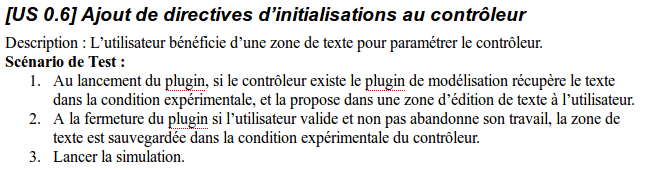
\includegraphics [width=130mm]{images/exempleUS.png}}
\captionof{figure}{Exemple de User Story}%\label{visina8}%      only if needed  
\end{minipage}

\section{Résultat du modèle type des cellules}
Voici les courbes obtenues après simulation d'un modèle avec le plugin IBM sur le logiciel GVLE du modèle type du la partie 2.1.2.

\begin{minipage}{\linewidth}% to keep image and caption on one page
\makebox[\linewidth]{%        to center the image
  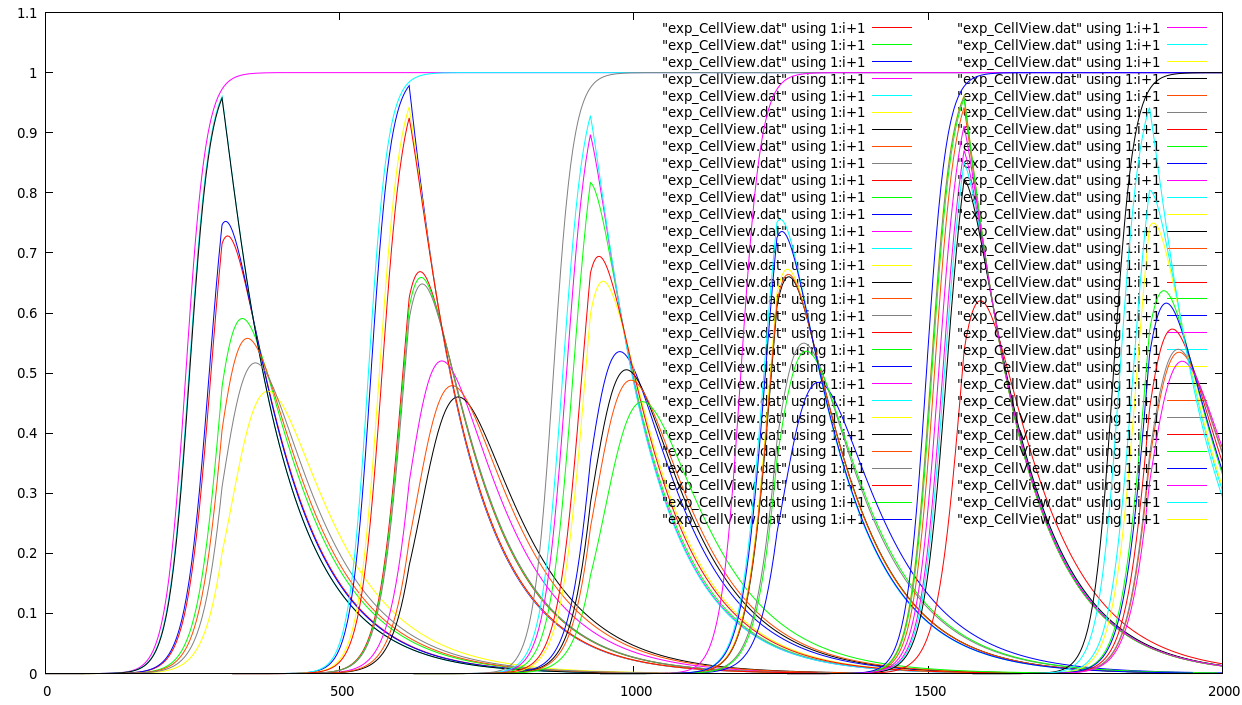
\includegraphics [width=120mm]{images/resultatIC.png}}
\captionof{figure}{Poids de chaque cellule vivante par rapport au temps}%\label{visina8}%      only if needed  
\end{minipage}

On remarque bien des vagues de 10 naissances de cellules puis la plus grosse reste vivante alors que les autres déclinent et meurt.

\section{Huit cas d'utilisation sur les 21 existants}
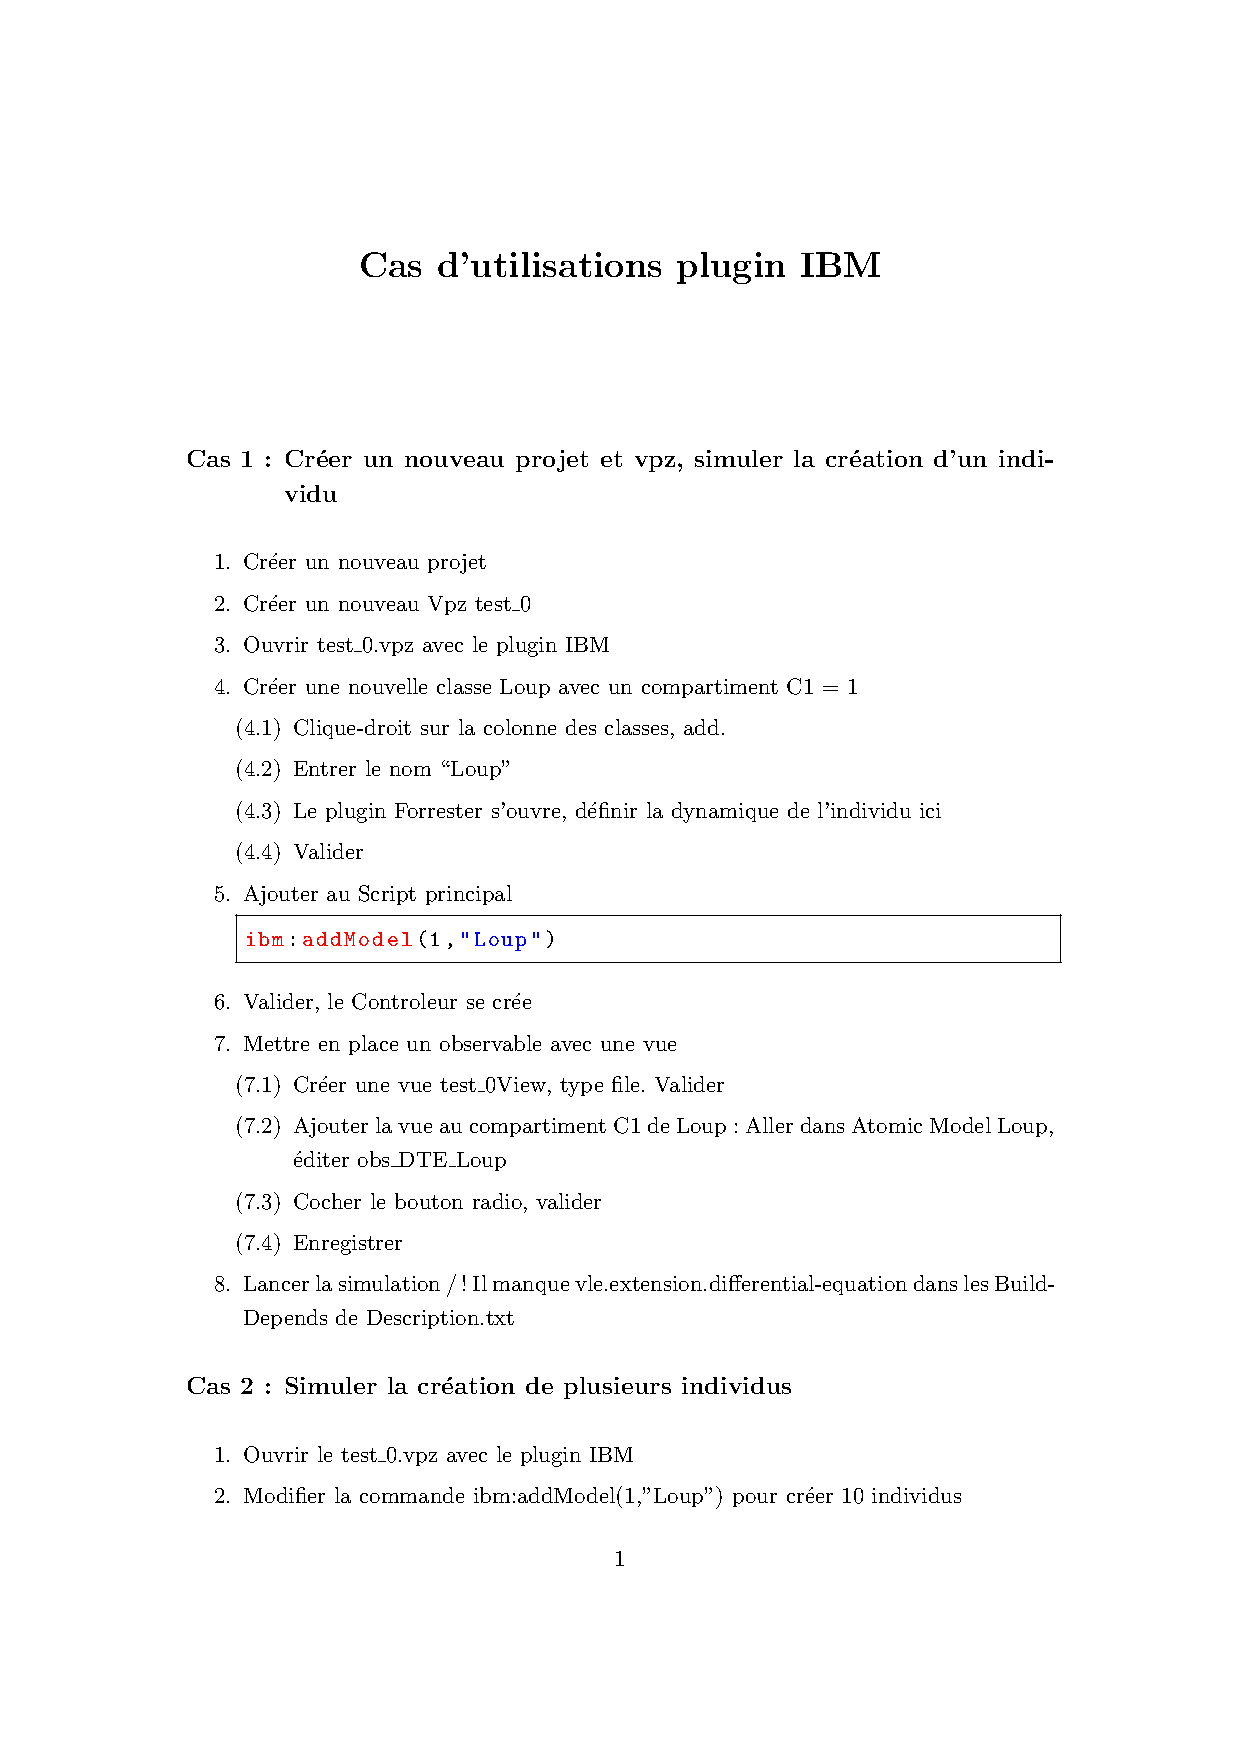
\includepdf[pages=1-3]{../CasUtilisation.pdf}